%\def\input@path{{..}}
\documentclass[a4paper,11pt]{kth-mag}
\nonstopmode
\usepackage[T1]{fontenc}
\usepackage{textcomp}
\usepackage{lmodern}
\usepackage[utf8]{inputenc}
\usepackage[swedish,english]{babel}
\usepackage{modifications}
\usepackage{comment}
\usepackage{tikz}
\usepackage{lipsum}
\usepackage{verbatim}
\usepackage{listings}
\usepackage{color}
\usepackage{minted}
\usepackage{graphicx}
\usepackage{comment} 
\usepackage{csquotes}
\usepackage{wrapfig}
\usepackage[pdfborder={0 0 0}]{hyperref}
\usepackage[doi=true,url=true]{biblatex}
\usetikzlibrary{matrix,shapes,arrows,positioning,chains, calc}

\newlength{\RoundedBoxWidth}
\newsavebox{\GrayRoundedBox}
\newenvironment{GrayBox}[1][\dimexpr\textwidth-4.5ex]%
   {\setlength{\RoundedBoxWidth}{\dimexpr#1}
    \begin{lrbox}{\GrayRoundedBox}
       \begin{minipage}{\RoundedBoxWidth}}%
   {   \end{minipage}
    \end{lrbox}
    \begin{center}
    
\begin{tikzpicture}%
       \draw node[draw=black,fill=black!10,rounded corners,%
             inner sep=2ex,text width=\RoundedBoxWidth]%
             {\usebox{\GrayRoundedBox}};
    \end{tikzpicture}
    \end{center}}


\pagenumbering{arabic}

\newmintedfile[gocode]{go}{ 
%linenos=true,
samepage=true,
fontsize=\footnotesize,
%xleftmargin=20pt 
}
\newmintedfile[jscode]{javascript}{ 
samepage=true,
fontsize=\scriptsize
}
\usemintedstyle{tango}

\addbibresource{bibfile.bib}
\counterwithout{section}{chapter}
\counterwithout{table}{chapter}
\counterwithout{figure}{chapter}
\counterwithin{table}{section}
\counterwithin{figure}{section}

\title{Proof of Work}

%\subtitle{An evaluation of proof of work as a DOS prevention method}
%\subtitle{A load measure approach to cryptographic mitigation of denial-of-service attacks}
\subtitle{A reputation based approach to cryptographic mitigation of denial-of-service attacks}
%\foreigntitle{Lorem ipsum dolor sit amet, sed diam nonummy nibh eui
 %             mod tincidunt ut laoreet dol}
\author{Fredrik Lilkaer, Christopher Teljstedt}
\date{Februari 2013}
\blurb{Bachelor's Thesis\\Supervisor: Douglas Wikström}
\trita{} %TRITA xxx yyyy-nn
\begin{document}
%\frontmatter
%\pagestyle{empty}
\removepagenumbers
\maketitle
\selectlanguage{english}
\newpage
\begin{abstract}
Lorem ipsum dolor sit amet, consectetur adipisicing elit, sed do eiusmod tempor incididunt ut labore et dolore magna aliqua. Ut enim ad minim veniam, quis nostrud exercitation ullamco laboris nisi ut aliquip ex ea commodo consequat. Duis aute irure dolor in reprehenderit in voluptate velit esse cillum dolore eu fugiat nulla pariatur. Excepteur sint occaecat cupidatat non proident, sunt in culpa qui officia deserunt mollit anim id est laborum.
\end{abstract}
\newpage
\section*{Statement of Collaboration}
Fredrik initiated the programming work on the testing software framework developed, including protocol, server structure and a ``normal service''- interface.
Christopher continued the work with an attacker web page, able to control an attack behaviour against the site. A monitor page was developed by Fredrik. Further improvements where developed in conjunction as need arose.

Christopher created the boilerplate of the document and wrote the initial introduction.
Both participated equally in respect to writing, analysis of results and final editing. The thesis is a collaborative effort.
\newpage  
\setcounter{section}{0}
\tableofcontents
\newpage
\section{Introduction}
The Internet continues to grow and has since a time back fulfilled it's early promise to enable a single source to be connected to several millions of geographically dispersed computers. However, as a consequence it has introduced security flaws of a new magnitude, allowing a single computer to potentially be attacked by millions of sources at once.

A popular attack is the Denial of Service\footnote{For a brief introduction to Denial of Service attacks please see section \ref{text:dos}} (DoS) attack, which aims to restrict or disrupt the availability of the service to its users.
One attempt to counter DoS attacks and to improve service survivability is a computational approach called Proof of Work (PoW).
Proof of Work is an economic scheme that requires a service requester to perform some work in order to access a service.
The concept was originally proposed by \citeauthor{DworkN92}\cite{DworkN92} as a way to counter e-mail spam by increasing the costs of sending spam, thus making e-mail spam economically unfeasible.
\citeauthor{DworkN92} originally called this a \emph{pricing function} since it effectively puts a price on the service to the client.
PoW was reinvented by \citeauthor{Back02}, who later proposed it as a DoS preventing method in \citetitle{Back02}. 

In this paper, we present a reputation based PoW problem difficulty scaling model and compare it to a simple load based scaler.

 
%and the idea is essentially to respond with a problem that is moderately hard to compute but easy to verify. They introduced this concept as a way to fight e-mail spam 
%In recent studies researchers have shown an increased interest in the Proof of Work (PoW) concept in order to prevent or mitigate the effects of a DoS attacks instead of fighting spam.

% The idea is to require the clients to solve an instance of a predefined problem in order to gain access to the server’s resources. To cope with a potential DoS attacks the level of difficulty of the problems is scaled proportionally with the amount stress that is put on the system. [källa på det här]


%\\
%Recently, researchers have shown an increased interest in the Proof of Work (PoW) concept in order to prevent or mitigate the effects of a DoS attack on such a system. The idea is to require the clients to solve an instance of a predefined problem in order to gain access to the server’s resources. To cope with a potential DoS attacks the level of difficulty of the problems is scaled proportionally with the amount stress that is put on the system. [källa på det här]

 % problem would then scale with the The solving of the problem would decrease the rate that each client would be able to issue requests to the server. This reduces the total number of requests that reach the content server in any given timeframe to a level l. l could be tuned to a level lower than the server’s inherent threshold of requests able to execute in said timeframe.
\section*{Background and Related Work}

One of the most significant threats in server security are Denial of Service (DoS) attacks. It is essentially a targeted effort to prevent a service from functioning properly by draining the underlying computer resources. There are different levels of the attacks which either can be targeted to exploit vulnerabilities in the TCP/IP-protocol, in the operation system that the server runs on or more specific implementations of the service. [källa på det här]

\\
\\
%Researches have shown Proof of Work to have mitigating the effects of a DoS attacks but. To cope with a potential DoS attacks the level of difficulty of the problems is scaled proportionally with the amount stress that is put on the system. [källa på det här]

 % problem would then scale with the The solving of the problem would decrease the rate that each client would be able to issue requests to the server. This reduces the total number of requests that reach the content server in any given timeframe to a level l. l could be tuned to a level lower than the server’s inherent threshold of requests able to execute in said timeframe.

%The Denial of Service (abbr. DoS) is a class of cyber attacks directed to attack the availability of a web service. The typical DoS attack exploits the server by generating excessive memory and/or CPU utilisation of the server. Popular examples include SYN spoofing attacks which triggers the server to allocate input buffers for connections that never complete initiation as well as SSL attacks in which the server CPU is overloaded with expensive public-key decryption calculations. 
			
%One of the big challenges when facing DoS attacks is to distinguish between a legitimate user and an attacker. One approach is to block senders of erroneous packages, but when malicious users pose as legitimate this method certainly fails. The objective is to ensure the availability of the service to the legitimate users without infeasible delays. 

\subsection*{Problem definition}
Proof of Work has been shown to potentially work as a prevention mechanism to at least mitigate the effects of a DoS attack\cite{subpuzzles}LÄGG IN ANNAN KÄLLA HÄR. However, scaling the problem difficulty with server load has proven to render problems so difficult that the problems induce a significant disruption to the legitimate client [VÅRA RESULTAT ELLER NGN ANNANS, KÄLLA PLIX]. Other problem with naive proof of work implementations such as hashcash is that it is largely CPU-bound\cite{hashcashbench}. This 


\begin{comment}
Proof of Work has been shown to potentially work as a prevention mechanism to at least mitigate the effects of a DoS attack without making an as assumption about the source.[källa] However, \citeauthor{LaurieC04} concluded in the paper \citetitle{LaurieC04}, that PoW on it's own, is not a feasible solution to fighting spam and denial of service attacks. This is because the classical implementation of Proof of Work does not seperate legitimate users from attackers. Hence, problems from a Proof of Work protected system would not discourage abusers of the system without having an unacceptable effect on legitimate users. 
\end{comment}
\subsection*{Problem statement} %Alternatively: (Presentation of the problem)?
% Since naive PoW difficulty scalers tend to 
\begin{itemize}
\item Can an individually adaptive Proof of Work scheme be optimised to penalise malicious behaviour while still enabling legitimate clients to access the service, thus improving performance versus a conventional load scaling system?

\item Is there a viable way to implement a Proof of Work system that maintains service, even to mobile users, while the system is under attack?

\end{itemize}

\begin{comment}
With the problem defined the question at hand is thus if it is possible to develop a Proof of Work protocol that is independent of client characteristics.
\begin{itemize}
\item Is there a viable way to implement a Proof of Work system so that the system's resources are accessable by a diverse variety of devices?

\item How should the protocol be optimised for low impact on legitimate client behaviour and high impact on malicious behaviour?

\item What advantages and disadvantages does proof of work concept bring in practice and in which applications could it be an improvement to current security?
\end{itemize}
\end{comment}
\subsection*{Purpose and method}
The purpose of this study is to research ways to improve the classical Proof of Work in such a way that legitimate users are less affected by the Proof of Work than the participants of a DoS attack. Furthermore find a way to dynamically scale the required proof of work when dealing with different hardware.
\subsection*{Scope and delimitations}
This study is explores a reputation based approach to scaling proof-of-work puzzle difficulties, thereby covering necessary theory of puzzle-based mechanisms specifically hash-reversal based puzzles. Furthermore, the study aims to cover explainations of the implemented protocol, simulation experiments and results of significance. 

There is various types of proof-of-work protocols as of recently. Hence, the study does not specifically aim to cover these but might be mentioned throughout the paper. 

\begin{comment}
Scope: \\
The coverage of this study ..... \\
The study consists of ..... \\
The study covers the ..... \\
This study is focus on ..... \\

Delimitations: \\
The study does not cover the ..... \\
The researcher limited this research to ..... \\
This study is limited to ..... \\
\end{comment}
\subsection*{Methodology}
\input{methodology}
\subsection*{Terminology}
Throughout this paper attackers or users with malicious intent will be referred to as \emph{adversaries}.
\emph{Client} and \emph{user} will be used interchangeably depending on the context where the term client tend to be more software oriented in contrast to user which usually is referred from an ``in system'' perspective.
%Technically an adversary is a client in the system, however if avoidable, an adversary will not be regarded as an user because adversaries does not seek to use the system's services as intended. 
An adversary is technically a client in the system, but will not be regarded as such throughout this paper, since the intentions of the adversary is to exploit and/or interrupt the service in contrary to the legitimate client. 
%however will not be regarded as a user, since an adversary intend to exploit and/or disrupt 

\subsubsection*{Miscellaneous Abbreviations}
A brief summary of used abbreviations follows:
\begin{itemize}
\item {\textbf{ SHA2}}: refers to the SHA256 secure hash algorithm\cite{sha2}.
\item \textbf{ Puzzle}: A problem instantiation of the problem type specified in the protocol. See section \ref{text:protodesc}.
\item \textbf{ Problem}: A general problem, may also refer to a Puzzle.
%\item \textbf{}
\end{itemize}
%\setcounter{section}{0}

\section{Theoretical approach}
%LINKZÄ http://conferences.sigcomm.org/co-next/2007/papers/studentabstracts/paper46.pdf se 2. THE PROOF-OF-WORK APPROACH
%
%https://www.ideals.illinois.edu/bitstream/handle/2142/17372/TechReport.pdf?sequence=3
%
% Puzzle-based defense mechanisms such as [41, 9, 20, 35, 26] try to correct the imbalance between the cost to the attacker for generating a request and cost to the server for processing a request by demanding a payment, in the form of a puzzle solution, from each client. In a typical puzzle-based scheme, a request must be accompanied by a proof of payment from the client. The payment may be in the form of computation or memory accesses that the client needs to perform to solve the puzzle. Since the amount of resources available to the attacker is limited (even if it is much more than that of the legitimate clients), the attacker will not be able to trivially amplify his attack. There are different kinds of schemes that build on this general principle. Laurie et al. [31] have analyzed proof-of-work schemes in the context of a spam deterrent mechanism and conclude that proof-of-work schemes do not work, because the cost involved for legitimate senders would be too high. However, their economic estimation contains a miscalculation. More importantly, their analysis considers fixed-cost puzzle schemes and does not analyze adaptive proof-of-work schemes proposed by recent DoS counter-measures.

Denial of Service attacks are often possible due to the relative price of a request, for an adversary often a single network packet\cite{gunter}. Puzzle-based proof-of-work limit an attacker's possibilities to impose a high work load on a server from a sole client by increasing the cost of each request. 

The RB-PoW scheme utilises a hash-reversal puzzle very similair to hashcash. The problem definition is a seed $P_i[j]$\footnote{For a precise definition of $P_i[j]$, $i$ and $j$, please see section \ref{text:protonot}}. The client needs to find $S_i[j]$ such that the computed hash $ h = H(S_i[j]||P_i[j])$ holds the property that the leading $d$ (issued difficulty) digits in the hex representation of $h$ are all equal to zero. It is computationally infeasible to find $x$  for a given $h$ such that $ h = \mbox{sha2}(x)$\cite{sha2}, consequently the only way to find $S_i[i]$ is by sequential trial. For $d_l = d + 1 $, only $\frac{1}{16}$ of solutions accepted for difficulty $d$ are accepted. The complexity of finding $S_i[j]$ is thus $O(16^d)$. This is however an amortized complexity, since one can be lucky and find a solution in the first hash test, or be forced to seek nealy the complete solution space. The actual running time is actually geometrically distributed with an expected outcome of $16^d$ trials before finding the solution, but the running time may be improved to approach a normal distribution with the introduction of subpuzzles\cite{subpuzzles}. The reputation based proof-of-work model uses subpuzzles to normalise expected solving times but also to scale problem difficulties. To 

The difference to hashcash is that RB-PoW uses SHA2 in place of SHA1, since it is a cryptographically stronger hash. 


The following sections will present server-side metrics needed to define client behaviour and explain assumptions made for a target application. 
We will precisely define the meaning of client behaviour in our model and finally carry on to develop and describe the reputation based proof-of-work model.

\subsection{Metrics}
%\footnote{See section \ref{tab:system}} %\footnote{See section \ref{tab:reputation} and \ref{tab:behaviourmodel}}
In order to establish a quantitative description of metrics required by the difficulty scaling model as well as simulation experiments
 this section will outline three sets of parameters referred to as quantifiers, observables and controllables. 

\subsubsection{Attack Quantifiers}
%In our Reputation Based Proof of Work system a DoS attack can be quantified by following sets of measurements: 

\emph{Service time} reflects measurement in the quality of a requested service by a client. Assuming that the service is web browsing the service time could be the time until a web page is completely transfered. If an adversary aims to mount a DoS attack the service quality during the attack can be measured by the average service latency for legitimate users. 

\subsubsection{Server Observables}
The difficulty of PoW problems handed out as a response to requests are based on a set of selected parameters that in different ways reflects the server's resource consumption.

\emph{Number of established connections:} keeps track of how many clients\footnote{This is actually the number of web sockets open on the server side.} that is currently connected to the server.

\emph{CPU load averages:} tell us whether the physical CPU utilization is over or under saturated. A perfect utilization is when the CPU is busy but no process is stalled. In general load average differ from CPU usage in two significant ways:
\begin{enumerate}
\item the CPU usage measures the instantaneous snapshot while load averages measure the trend in CPU utilization.
\item the CPU usage only measures how much was active during measured timeframe while load averages take all demands for CPU into account.
\end{enumerate}
If the server has four CPUs running and the reported load average is 4.00 then the CPUs are perfectly utilized\cite{cpu}.

\emph{Request rate} is the quantified amount of requests for a service that a single \emph{client} or a \emph{group of clients} asks for. This measurement is slightly modified to measure the average time between requests to show the amount servicing required by each client and the average of all clients in a given time-frame. By introducing a rating scheme that weights the individual requesting rate of a client with the average request rate of all clients the Reputation System can hand out problems scaled to the behaviour of each client. Thereby limiting the amount of service to a client with malicious behaviour and furthermore giving a natural limit to a DoS attack.


\subsubsection{Server Controllables}
The server resources is managed by the reputation behaviour model, generally it has two settings that can be regulated.
Firstly, \emph{Puzzle Difficulty}, the difficulty of a puzzle is based on parameters in Server Observables. However, the scaling of puzzles can be tuned to respond more harshly or forgiving based on the parameters.

Secondly, \emph{Connection Time-out} is used to control the lifetime a connection. This could be a finite duration meaning that if no solution is sent back to the server within the connection lifetime the connection will be closed.
However, in the scope of the simulation experiments this duration is set to infinite. %, see Attack Model below for explanation of our assumptions about the attacker. 

%\subsection{Attack Model}
\subsection{Assumptions}
\subsubsection{Attack model}
In this section, the attack model of the simulation experiment will be described.
In order to specify an attack model and to simulate an attack, some assumptions regarding the adversary are required.
Assumptions made enable us to test a DoS mitigation scheme in the application layer; if any assumption does not hold the protection can be circumvented by an attack through a lower abstraction layer\footnote{Abstraction layer in the OSI model}. 
We assume a server \emph{Server}, a network with clients \emph{$\{C_i\}$}, and adversary \emph{Ad}.
\\
\\
\noindent \textbf{Assumption 1} \indent \emph{Ad} cannot modify any packets sent between \emph{$C_i$} and \emph{Server}.
\\
\\
This is necessary to assume, in particular that it cannot modify legitimate users packets. If Assumption 1 does not hold and packets can be modified then a denial-of-service attack can be initiated simply by corrupting all packages thus rendering any PoW protocol ineffective.
\\
\\
\\
\noindent \textbf{Assumption 2} \indent \emph{Ad} cannot delay any packets sent between \emph{$C_i$} and \emph{Server}.
\\
\\
By similar reasons as Assumption 1 we must assume that the adversary cannot delay other clients' packets. If Assumption 2 does not hold and an adversary can delay packets arbitrarily then the she can mount a denial-of-service attack without draining the resources of the server itself.
\\
\\
\\
\noindent \textbf{Assumption 3} \indent \emph{Ad} cannot oversaturate the transfer layer\footnote{Transfer layer of the OSI model} or network layer\footnote{Network layer of the OSI model} of the \emph{Server}.
\\
\\
An adversary must be able to initiate a denial-of-service attack by large amount of requests to the server. However, we must also assume that the adversary cannot bring down the server by simply over-saturating the server ports or network with sheer volume of the adversary's requests.
\\
\\
\subsubsection{Environment}
\noindent \textbf{Assumption 4} \indent We will assume that every action the server performs have unit cost, the assumption does not lessen generality, since an external difficulty scaler could be added to each action the server performs.
\\
\\
\noindent \textbf{Assumption 5} \indent We will assume that the server is dimensioned to handle normal load.
\subsection{Behaviour model}\label{tab:behaviourmodel}
In the context of our reputation system, behaviour is defined as the measured time between requests sent to the server. Furthermore, both historical data and close to real-time data are taken into account by the use of a rolling average. However, there is two fundamental differences in the way that global behaviour is computed in comparison to the individual behaviour of a client. The first and most important difference is that the individual client behaviour is rated based on it's own frequency of requests, while the global behaviour is based on the frequency between the requests of all clients. 

A perhaps a more subtle difference is how much weight the historical behaviour should have. The weight of historical behaviour impacts the rate of change. Thus a higher weight gives a more stable and slower moving measurement of the behaviour. Hence, more fitting for the defining the general behaviour of clients on the server. While a lower weight tend to be closer to real-time measurement thus befitting the individual behaviour of a client.

\subsection{Reputation Mechanism as a Difficulty Scaler}
We propose a conceptually simple yet in practice effective reputation system. A client is rated based on historical and current behaviour. The reputation mechanism distributes proof of work problems with a difficulty dependant on the individual client behaviour compared to the global average behaviour as well as server load. 

The basic idea of the RB-PoW scheme is that the server is dimensioned to handle normal load. If the server load is beneath \emph{cpu\_thres}, the server is in a normal state and no PoW scheme needs to be applied. If server load is above {\em cpu\_thres}, PoW may be activated, suspecting all clients as possible adversaries [SOURCE HÄR]. Another foundation of the RB-PoW model is an assumption that legitimate clients utlises a lower request rate than a malicious user. so if the server is under attack we compare the behaviour ( access time ) of the client against global average. If extremely favourable, client may get a free ticket to the zoo, and if extremely taxing on the server client gets an extremely hard problem.  ;)

\newpage
\section{System Architecture}
Since one requirement of a Proof of Work system is that it minimises differences between a wide variety of devices appearing in the wild we needed to support both desktop and laptops with different operating systems as well as cellphones and tablets.
In order to minimise the development effort and maximise maintainability of the code base, a multi platform solution was sought for the client part of the demo application. 

A web based solution makes the perfect portable application, however the web is not inherently stateful and quite badly imitates an application server which keeps a constantly open socket connection with connected clients. The advent of websockets turn the whole thing around, with the help of DoS nice fellas we were able to write a truly multi-platform PoW client in html and javascript which maintains the generality and plasticity of a natively written socket based application. The javascript implementation for handling th protocol is quite simple:
\jscode[firstline=57, firstnumber=57, lastline=84]{../pow.js}
The solution finding part also need to be present:
\jscode[firstline=26, firstnumber=26, lastline=49]{../pow.js}
To trigger a request to be sent to the server we build the following function which is then registered to the onclick event of a button in the web gui:
\jscode[firstline=100, firstnumber=100, lastline=105]{../pow.js}

For the server side we choose to use Googles novel programming language go(\citeurl{golang}). The real strengths of golang in this context is actually not performance nor simplicity\footnote{But the expressiveness, clarity and performance of go programs is not to be dismissed.} but rather it's standard libraries, which in other contexts may appear immature. Golang actually has standard libraries for both http template generation, web serving as well as websockets. This package makes for an ideal platform for an application that needs to deliver the client application\footnote{HTML, CSS, Javascript and all that magic that make stuff happen in the browser} to potential clients as well as servicing clients requests in the model application reachable through the websocket interface. 

To further ease our programming task, we choose to communicate over the websocket with a single message type which is (de-)serialised (from) to JSON. JSON is natively supported in the Javascript client, and the golang websocket library supports JSON (de-)serialisation which makes for a nice pairing where we have to write absolutely no byte parsing for our protocol.
\gocode[firstline=35, firstnumber=35, lastline=40]{../conn.go}

\subsection{The Reputation Based Puzzle Protocol}
\subsubsection{Protocol notation}
\subsubsection{Puzzle construction and protocol parameters}
\subsubsection{Protocol description}
Now let us describe the details of our proposed reputation based puzzle protocol between client and server. Prior to initiating protocol \textbf{P} the client $C_i$ starts by requesting for a service $R_i$ to the server. The server responds with a packaged set of sub-puzzles $\phi_i$. If the reputation system deems the server to not being under attack i.e. under normal server operation this package will be the empty set, indicating that no puzzles are being distributed. Hence, the client will ''solve'' this empty set with no effort and then respond back to the server.\footnote{This is a design decision that can be questioned. Some might say that the handshaking process with empty sets could bring unneccesary load on the server. However, empty sets will only be distributed when pressure on the server is low thus the extra verification can be afforded.} The server will then verify the solution for $\phi_i$ and grant access to $R_i$ of protocol \textbf{P}.

\begin{figure}[H]
	\begin{center}
		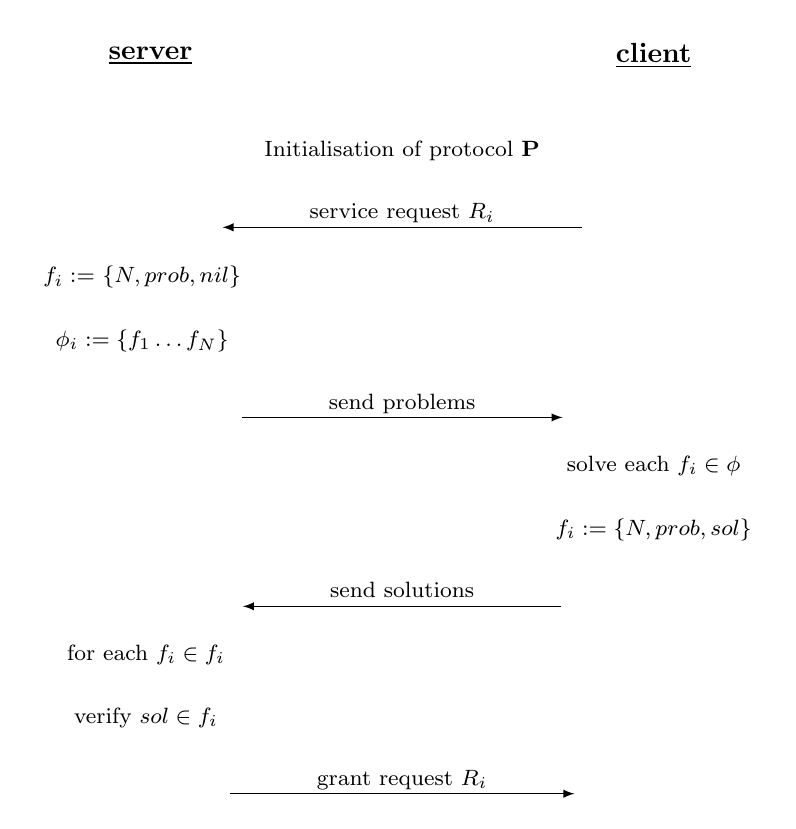
\begin{tikzpicture}

		\footnotesize
		\matrix (m)[matrix of nodes, column  sep=0mm,row  sep=4mm, nodes={draw=none, anchor=center,text depth=0pt} ]{
		\textbf{ \underline {\normalsize server}} & & \textbf{\underline {\normalsize client}}\\[0mm]
		& & \\
		& Initialisation of protocol \textbf{P}& \\
		& service request $R_i$& \\
		$f_i:=$ $\{N,prob,nil\}$ \hfill \\
		$\phi_i :=  \{f_1\dots f_N\} $ \hfill \\
		& send problems & \\
		& & solve each $f_i \in \phi$ \\
		& & $f_i := \{N,prob,sol\}$ \\
		& send solutions & \\
		for each $f_i \in f_i$ & & \\
		verify $sol \in f_i$ && \\ 
		& grant request $R_i$& \\
		};
		\draw[shorten <=-1cm,shorten >=-1cm,-latex] (m-4-2.south east)--(m-4-2.south west);
		\draw[shorten <=-1cm,shorten >=-1cm,-latex] (m-7-2.south west)--(m-7-2.south east);
		\draw[shorten <=-1cm,shorten >=-1cm,-latex] (m-10-2.south east)--(m-10-2.south west);
		\draw[shorten <=-1cm,shorten >=-1cm,-latex] (m-13-2.south west)--(m-13-2.south east);
		\end{tikzpicture}
		\vspace{10pt}
		\caption{Diagram of Proof of Work protocol}\label{tab:protocol}
	\end{center}
\end{figure}
\\
\\
If the reputation system deems the server to be under attack the difficulty of the problem set of request $R_i$ will be decided by the historical and current behaviour of client $C_i$. 
\\
\\
The client behviour can generally be divided into three cases:
\begin{itemize}
\item the client $C_i$ behaves in a comparable manner to the general behaviour of all users and the request $R_i$ is responded with a problem difficulty suitable to server load.
\item the client $C_i$ requests lesser resources compared to the general behaviour and the request $R_i$ is responded with a problem difficulty easier than the general difficulty.
\item the client $C_i$ requests more resources compared to the general behaviour and the request $R_i$ is responded with a problem difficulty harder than the general difficulty.
\end{itemize}

To prevent an attacker from reusing solutions for multiple requests the problem set $\phi_i$ is stored in memory on the server.
[lite mer information om generering av problem. Varje problem är relativt unikt för varje request osv]

\subsubsection{Reputation System}
\section{Tuning the Reputation System} \label{tab:system}
\subsection{Interesting Parameters}
\subsection{First Model}
\subsection{Reputation based on Request Rate Behaviour}
\newpage
\section{Simulation Experiments}
The reputation based PoW system's architecture and load management mechanism was tested by conducting series of simulated experiments using custom made web-based population-simulation interface. The configuration parameters of the experiments are described in detail in section \ref{text:setup}.
% is shown in Figure [NUMMER].

In the experiments, a fixed set of legitimate users was programmed to send requests for a service from a single server. To simulate a legitimate population each client was programmed to send the requests with stochastic based delays and thereby simulating the unpredictable rate of requests. Each request was also programmed to perform a fixed load on the server side to simulate the execution of a service. As a result a normal work load on the server was simulated. 
%If the server accepts the solution, it offers the client some meaningless cpu cycles in order to simulate a request:
\begin{minted}[fontsize=\footnotesize]{go}	
for i := int64(0); i < 250000000; i++ {
	//simulate some server load (~80 ms)
}
\end{minted}
The requests of legitimate users was mixed with a larger population of adversaries to mount a DoS attack. The adversaries was programmed to have lesser to zero delay in-between requests, thus forcing the server to service more requests than a legitimate user. 

A custom made web-based monitor was used to investigate how well the RB-PoW system performed under different scenarios. The monitor uses real-time graphs to outline information about CPU utilization, requests rates and the time to solve PoW puzzles. In each run we studied the service time for adversaries, legitimate and mobile users to see how the protection system affected each type of behaviour. Control parameters such as number of attacking connections and settings for delays was changed between experimental runs, as-well as the parameters for server's internal reputation mechanism.

The goal of the experiments was to examine how well the reputation based PoW architecture performed in mitigating DoS attacks and at the same time serving legitimate users and users with lesser hardware. The degree of effectiveness from the experiments conducted was determined by following observations:

\begin{itemize}
\item A comparison of how many attacking connections that was required to launch DoS attacks with comparable levels of performance degradation, with and without reputation based PoW.

\item How much legitimate users and users with lesser hardware was affected by DoS attacks, with and without reputation based PoW protection.
\end{itemize}

%The attack model is based on assumptions necessary to make any protection scheme in 

%\subsection{Assumptions}

\subsection{Setup}
The simulation experiments resulted in benchmarking the Reputation Based Proof of Work with the initially proposed Proof of Work protocol. In this section, the set-up of the benchmarks will be presented.
\label{text:setup}
\subsubsection{The legitimate users} 
The legitimate users had to be set fixed amount. By being consequent, a fair comparison could be done simulating the same normal work load on the server through all the simulations. The benchmarks was run with 100 legitimate users, each being set to having a normally distributed access times expected to ten seconds with a fifteen second standard deviation. Consequently, the most probable delays would vary between between zero to forty seconds.
\\
\subsubsection{Mobile user}
The mobile users where set to have the same behaviour as the legitimate users in respect to request rate. Due to a relative lack of testing hardware the cellphones clients where only four by number, running on a single device. 
\\
\subsubsection{The attackers} 
The simulation experiment will test the solution for two different kinds of malicious behaviour, both seeking to drain the server resources.

\emph{Flooding Behaviour}: The attackers try to submit as many requests as possible, solving the problems as fast as possible regardless if proof-of-work is activated. The test set-up consists of seventeen Quad Core Q9550 2.83Ghz machines running Ubuntu operative system each handling four client processes in parallel.

\emph{Draining Behaviour}: The attackers try to have many connections open in parallel, even if it means an increased number of contexts switches and longer solving time for each problem when proof-of-work is activated. This set-up consist of twelve equally specified machines each running 40 clients in parallel.

The server load is in fact only affected by the total request rate, but the reason to test both flooding as well as draining is to examine performance of RB-PoW under different circumstances, since a lower individual request rate among adversaries may well disguise concerned adversary amidst legitimate users.



\section{Results}
% Column settings for tables (array,dcolumn)
\newcolumntype{d}{D{.}{.}{-2}}
\newcolumntype{e}{D{.}{.}{-3}}
\begin{comment}
  \begin{table}[H]
    \centering
    \tiny
    \begin{tabular}{lcccccccc} \toprule
      \multicolumn{1}{c}{Prot. model} & \multicolumn{3}{c}{Attackers} & \multicolumn{2}{c}{Legitimate users} & \multicolumn{2}{c}{Mobile devices} \\
      %\unitfrac{ml}{min} & \multicolumn{2}{c}{mS} & & & \multicolumn{2}{c}{mmHg} & \textcelsius  \\ \midrule
      \multicolumn{1}{c}{} & \multicolumn{1}{c}{Pop. size} & \multicolumn{1}{c}{Solving} & \multicolumn{1}{c}{Service} & \multicolumn{1}{c}{Solving} & \multicolumn{1}{c}{Service} & \multicolumn{1}{c}{Solving} & \multicolumn{1}{c}{Service}  \\ \toprule
      None & 120x7  & 0.57$\pm$0.02 &  19861.19$\pm$375.23 & 0.48$\pm$0.05 & 19965.45$\pm$1286.18 & 16.87$\pm$7.64 & 20800.60$\pm$3202.62     \\ \bottomrule
    \end{tabular}

    \caption{No protection}\label{tab:noprot}

  \end{table}
\end{comment}

We performed two sets of experiments to design to test and study the effectiveness of RB-PoW in comparison to classical PoW;
\begin{itemize}
\item \emph{Server Flooding Attacks:} in this experiment, the server was flooded with adversaries programmed to have no delays between requests.

\item \emph{Server Draining Attacks: in this experiment, the server was drained by having a large amount of adversaries faking to be legitimate users by having identical delays as the legitemate users.} 
\end{itemize}

\subsection{Mitigation against Server Flooding}
  \begin{table}[H]
    \centering
    \tiny
    \caption{Results from simulating server flooding. All time measurements in milliseconds (ms). Attacker population size is seventeen computers simulating four clients each. The results are the mean of sample data with a 99\% confidence level that the population mean is within the interval. }\label{tab:flooding}

    \begin{tabularx}{1.05\textwidth}{lcccccccr{5cm}} \toprule
      \multicolumn{1}{c}{\textbf{Prot. model}} & \multicolumn{3}{c}{\textbf{Attackers}} & \multicolumn{2}{c}{\textbf{Legitimate users}} & \multicolumn{2}{c}{\textbf{Mobile devices}} \\
      %\unitfrac{ml}{min} & \multicolumn{2}{c}{mS} & & & \multicolumn{2}{c}{mmHg} & \textcelsius  \\ \midrule
      \multicolumn{1}{c}{} & \multicolumn{1}{c}{Pop. size} & \multicolumn{1}{c}{Solving} & \multicolumn{1}{c}{Service} & \multicolumn{1}{c}{Solving} & \multicolumn{1}{c}{Service} & \multicolumn{1}{c}{Solving} & \multicolumn{1}{c}{Service}  \\ \toprule
      % None & 80x6  & 0.67$\pm$0.03 &  11906$\pm$280.7 & 0.49$\pm$0.05 & 12011$\pm$816 & 14.7$\pm$2.23 & 11221$\pm$1843     \\ 
      PoW & 17x4  & 1266$\pm$9 & 1794$\pm$12 & 3129$\pm$98 & 3652$\pm$99 & 31959$\pm$4576 & 32488$\pm$4556    \\
      RB-PoW & 17x4 & 1875$\pm$43 & 2312$\pm$43 & 267$\pm$13 & 582$\pm$22 & 2975$\pm$1031 & 3469$\pm$1103   \\ \bottomrule
    \end{tabularx}

  \end{table}


\subsection{Mitigation against Server Draining}

  \begin{table}[H]
    \centering
    \tiny
    \caption{Results from simulating server draining. All time measurements in milliseconds (ms). Attacker population size is twelve computers simulating fourty clients each.  The results are the mean of sample data with a 99\% confidence level that the population mean is within the interval.}\label{tab:draining}

    \begin{tabularx}{1.05\textwidth}{lcccccccr} \toprule
      \multicolumn{1}{c}{\textbf{Prot. model}} & \multicolumn{3}{c}{\textbf{Attackers}} & \multicolumn{2}{c}{\textbf{Legitimate users}} & \multicolumn{2}{c}{\textbf{Mobile devices}} \\
      %\unitfrac{ml}{min} & \multicolumn{2}{c}{mS} & & & \multicolumn{2}{c}{mmHg} & \textcelsius  \\ \midrule
      \multicolumn{1}{c}{} & \multicolumn{1}{c}{Pop. size} & \multicolumn{1}{c}{Solving} & \multicolumn{1}{c}{Service} & \multicolumn{1}{c}{Solving} & \multicolumn{1}{c}{Service} & \multicolumn{1}{c}{Solving} & \multicolumn{1}{c}{Service}  \\ \toprule
       %None & 120x7  & 0.57$\pm$0.02 &  19861$\pm$375 & 0.48$\pm$0.05 & 19965$\pm$1286 & 17$\pm$7.64 & 20801$\pm$3203     \\ 
      PoW &  12x40  & 12700$\pm$199 & 14377$\pm$210 & 2616$\pm$119 & 3707$\pm$145 & 59119$\pm$14150 & 61005$\pm$14175    \\
      RB-PoW & 12x40 & 14615$\pm$380 & 15371$\pm$383 & 4555$\pm$332 & 5206$\pm$345 & 29940$\pm$13426 & 30753$\pm$13490   \\ \bottomrule
    \end{tabularx}
  \end{table}

\section{Conclusions}
In this paper, we have explored the possibilites of a reputation based proof-of-work protocol in mitigating DoS attacks. We have presented the RB-PoW protocol, an experimental architecture and tested the protocol with a web-based simulation interface. Furthermore, we presented results of two simulation experiments, server flooding and server draining with two types of implementations; classical proof-of-work and the proposed reputation based proof-of-work. The results from these simulation experiments will be brought to discussion in following paragraphs with the goal of answering the initial problem statements:
\\
\\
\\
\textbf{Server flooding}
\vspace{7pt}
\\
The results of simulating server flooding, see table \ref{tab:flooding}, shows that the RB-PoW protocol is a vast improvement to mitigating DoS flooding attacks in comparision the the classical PoW. It is interesting to note that the RB-PoW perform better in all three user-type cases. The most significant improvement was to the mobile users where the service time was improved by approximately 900\%. 

This finding was unexpected and suggests that PoW in its classical implementation is very primitive.
There are several possible explanations for this result and the most orenous reason is likely to be the fact that the classical PoW does not in any way seperate legitimate users from adversaries.
There are, however, other possible explanations. It may in fact be the result of inadequate tuning of the PoW protocol. Although, it does not explain the much lesser impact on legitimate clients in which RB-PoW had approximately a 130\% improvement over the classical protocol.
\\
\\
\textbf{Server flooding}
\vspace{7pt}
\\



\subsection{Feasibility}
\subsection{Statistical Confidence}
An important question of our study is, \emph{when do we trust our data?} The results presented in Section \ref{result} was collected from the simulation experiments run through the web-based simulation interface. The data was collected as samples during a certain time-frame during the experiments, dividing data into the categories of \emph{adversaries}, \emph{legitimate users} and \emph{mobile device users}. However,  can we be certain that the calculated averages of our samples represent the average of the whole population?

The answer lies in statistical mathematics. To bring confidence in the presented results it is important that a average of the sample data can, with a certain propability, be found within a interval of confidence, also known as confidence interval. Hence, knowing this interval enables the possiblity to infer that the average of one sample is significantly different from another, as long as the confidence interval of the averages do not overlap.

One fundamental requirement of finding these confidence intervals is that the distrubution of the samples is known. However, the distribution of our the result data in our simulation experiments is likely a sum of pascal and unknown distributed variables. Because of the uncertainty a bit of magic is required to solve this problem. 

\subsubsection{Arithmetic Averages Have a Bit of Magic}
That bit of magic is the \emph{Central Limit Theorem}. The theorem states that, given a sufficiently large sample of indentically distributed independent variables,\footnote{The central limit theorem generally takes effect when samples is larger than 30.}, each with a well-defined mean and well-defined variance\footnote{This implies that both the mean the variance should be finite.}, will be approximately normally distributed\cite{gunnar}.

From this theorem two implications can be drawn that is relevant for our test data:
\begin{itemize}
\item A random sample scan be taken from any population, in our case samples of the simulation experiments, even if the simulation data is not normally distributed and assume it to be approximately normally distributed.

\item The theorem also allows assumptions to be made about the sample data of the simulation regardless of the entire simulation data. Thereby, an interval estimation can be made about the true average of the simulation data with only sample data.
\end{itemize}

 \subsubsection{Confidence in Test Results}
The probability that the average of whole population falls within the interval of the result data is either 1 or 0 - the interval captures the average or it doesn't\cite{gunnar}. However, with a 99\% confidence it is safe to assume that the average of the whole population actually falls within the confidence interval of the result data. 


\subsection{Lessons learned}
\subsection{Suggested Directions for Future Research}

Optimise parameters used in scaling model

Explore the possiblities of non-linear difficulty scaling based on client behaviour. 

In future investigations it might be possible to use a different X in which ...... 

Further studies, which take these variables into account, will need to be undertaken.

\
\begin{comment}
\begin{figure}[ht]
\begin{center}
And here is a figure 
\caption{\small{Several statements describing the same resource.}}\label{RDF_4}
\end{center}
\end{figure}


that we refer to here: \ref{RDF_4}
\end{comment}
\printbibliography
\end{document}
